\documentclass[12pt, a4paper, oneside]{ctexart}
\usepackage{amsmath, amsthm, amssymb, bm, color, graphicx, geometry, hyperref, mathrsfs,extarrows, braket}

\linespread{1.5}
\geometry{left=2.54cm,right=2.54cm,top=3.18cm,bottom=3.18cm}
\newenvironment{problem}{\par\noindent\textbf{题目. }}{\bigskip\par}
\newenvironment{solution}{\par\noindent\textbf{解答. }}{\bigskip\par}
\newenvironment{note}{\par\noindent\textbf{注记. }}{\bigskip\par}

% 基本信息
\newcommand{\dt}{\today}
\newcommand{\sj}{离散数学}
\newcommand{\vt}{吴天阳 2204210460}

\begin{document}

\pagestyle{empty}
\vspace*{-20ex}
\centerline{\begin{tabular}{*3{c}}
    \parbox[t]{0.3\linewidth}{\begin{center}\textbf{日期}\\ \large \textcolor{blue}{\dt}\end{center}} 
    & \parbox[t]{0.3\linewidth}{\begin{center}\textbf{科目}\\ \large \textcolor{blue}{\sj}\end{center}}
    & \parbox[t]{0.3\linewidth}{\begin{center}\textbf{姓名,学号}\\ \large \textcolor{blue}{\vt}\end{center}} \\ \hline
\end{tabular}}
\vspace*{4ex}

\paragraph{第八章}

\paragraph{4.}\begin{proof}
    中间小正方形的左上角度为$3$的结点记为$v_1$,在$(a)$左图中,中间小正方形左下角度为$3$的结点记为$v_2$,$(a)$右图中,中间小正方形右下角度为$3$的结点记为$v_3$,则$d(v_1,v_2)=1$,而$d(v_1,v_3)=2$,故$(a)$左图与$(a)$右图不同构。

    记右下角有自环的结点为$v_1$,$(b)$左图中,右侧度为$4$的结点记为$v_2$,$(b)$右图中,左侧度为$4$的结点记为$v_3$,则$d(v_1,v_2)=1$,而$d(v_1,v_3)=2$,故$(b)$左图与$(b)$右图不同构。
\end{proof}
\paragraph{5.}\begin{proof}

    (1). 五个结点的自补图如下:

    \centerline{
        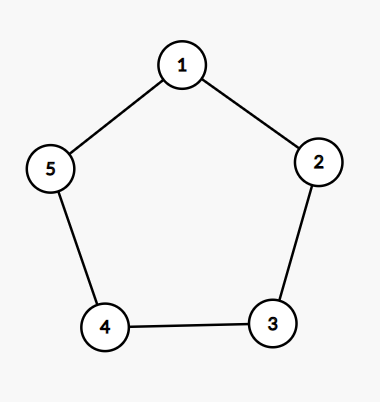
\includegraphics[width=0.3\textwidth]{graph1.png}
        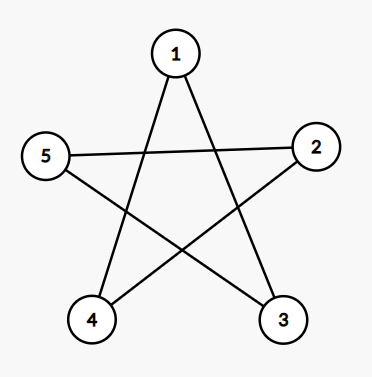
\includegraphics[width=0.3\textwidth]{graph2.png}
    }

    (2). 没有三个结点的自补图,因为三个结点的完全图边数为$\frac{3\cdot 2}{2} = 3$,为奇数,设图$G$为包含三个节点的图,边数为$n$,由于自补图边数必须相同,则完全图中的边数应为$2n$,与$3$为奇数矛盾,故没有三个结点的自补图。

    四个结点的自补图如下:

    \centerline{
        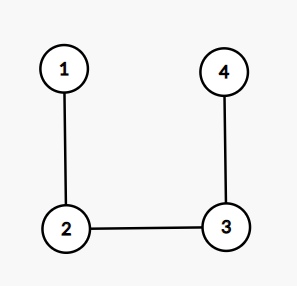
\includegraphics[width=0.25\textwidth]{graph3.png}
        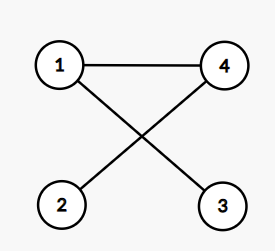
\includegraphics[width=0.25\textwidth]{graph4.png}
    }

    (3). 设$G$为自补图,$G$的边数为$n$,由于$G$同构于它的补图$G'$,则$G'$中的边数也为$n$,又由于$G$和$G'$中的边的并为完全图中的边数,则完全图中的边数为$2n$,故它对应的完全图的边数必然为偶数。
\end{proof}

\paragraph{6.}
\begin{proof}
    设组内一共有$n$个人,将每个人视为一个结点,朋友关系视为一条无向边,由于每个人不能和自己做朋友,两个人之间有且仅有一个朋友关系,所以此图没有重边和自环,故为简单图,且每个人朋友个数等价于人所对应的结点的度。

    反设,不存在两个人在组内有相同个数的朋友,即任意两个结点的度都不相同,由于简单图中结点的度必须在$0$到$n-1$之间,由于这正好也有$n$个数,故结点的度和$0,1,\cdots, n-1$构成双射,则一定存在一个结点的度为$n-1$,即它与其他所有结点都相邻,但这与图中存在一个度为$0$的结点矛盾。

    综上,一定存在两个人在组内有相同个数的朋友。
\end{proof}
\paragraph{10.}\begin{proof}
    反设$G$不是连通图,则存在$v_i\in G$,使得$\forall v_j \in V(G),\ v_i\neq v_j$,$d(v_i,v_j) = \infty$,即$v_i$与其他所有点都没有连边,则
    \begin{equation*}
        \begin{aligned}
            &m\leqslant \frac{n(n-1)}{2}-(n-1)\\
            \Rightarrow&\ m\leqslant \frac{(n-1)(n-2)}{2}
        \end{aligned}
    \end{equation*}
    与$m > \dfrac{1}{2}(n-1)(n-2)$矛盾。
    
    故$G$为连通图。
\end{proof}

\end{document}
